\documentclass[conference]{IEEEtran}
\usepackage{cite}
\usepackage{amsmath,amssymb}
\usepackage{graphicx}
\usepackage{booktabs}
\usepackage{array}
\usepackage{algorithm}
\usepackage{algpseudocode}
\usepackage{url}
\usepackage{xcolor}
\usepackage[hidelinks,pdfusetitle]{hyperref}
\graphicspath{{../figs/}}
\newcolumntype{L}[1]{>{\raggedright\arraybackslash}p{#1}}
\newcommand{\contactemail}{i232538@nu.edu.pk}
\hypersetup{pdfauthor={Muhammad Abdullah Aamir, Muhammad Ibrahim Kiani}}

\begin{document}

\title{Prompts Are Not Policies: Deterministic Pre-Execution Gating for Language-Model Agents Acting on Network Traffic}

\author{\IEEEauthorblockN{Muhammad Abdullah Aamir$^{\ast}$ and Muhammad Ibrahim Kiani}
\IEEEauthorblockA{Department of Data Science, FAST-NUCES, Islamabad, Pakistan\\
$^{\ast}$\contactemail}}

\maketitle

\begin{abstract}
Tool-using language-model agents are usually given their operating policy as text in the system prompt, which leaves compliance to the model. We test that arrangement for an agent that allows, blocks or rate-limits network flows labelled by an encrypted-traffic classifier. A 4-bit Llama-3.2-3B agent answered 100 scenarios once, and its proposals were replayed under five enforcement conditions. With the policy in the prompt alone, 30 proposals executed as violations: the agent carried out all 25 forbidden operator requests and followed 3 of 25 injected notes. A deterministic gate that checks each tool call before execution reduced violations to 6 (95\% CI of the paired difference 17.7--30.4 points), stopped every injection and kept 97.9\% of completed tasks, at a median 3.6\,$\mu$s per decision. Returning the rejection reason for one retry recovered 4 of 25 rejected tasks but produced one new violation. All violations that passed the gate traced back to mislabelled flows, which no rule on the agent side can correct.
\end{abstract}

\begin{IEEEkeywords}
Language-Model Agents, Policy Enforcement, Tool Use, Prompt Injection, Runtime Verification.
\end{IEEEkeywords}

\section{Introduction}

Language models now act through tools: they emit structured calls that change external state, a pattern established by interleaved reasoning and acting \cite{yao2023react} and by models trained to decide when to call an API \cite{schick2023toolformer}. Once an agent can change state, the question becomes which changes it is allowed to make. Benchmarks for tool-agent-user interaction show that agents given a written policy still break it in a large share of episodes \cite{yao2025taubench}, and recent studies document violations that occur even when the requested action looks reasonable from the visible context \cite{wu2026policyinvisible}. Untrusted content that reaches the model through tool outputs adds a second failure path, since text injected into the context can redirect the agent \cite{greshake2023,debenedetti2024agentdojo}.

Two families of defence have emerged. Model-side defences add another model that reviews actions in context \cite{kang2026policyguard,chen2025shieldagent}, at a measurable cost in calls and in task success \cite{sah2026verifier}. Code-side defences compile policy into checks that run before a tool executes \cite{zwerdling2025,wang2026agentspec} or restructure the agent so that untrusted data cannot alter control flow \cite{debenedetti2025camel}. Most evaluations of both families use customer-service, web or code domains. Network operations, where agents are already proposed for configuration and management \cite{wang2024netconfeval,wang2025confucius,adanza2026}, differ in two ways: a single mistaken action can affect every packet of a flow, and the fact that determines whether an action is allowed, the application behind an encrypted flow, is supplied by a classifier rather than read from a database.

We therefore study a small agent that manages individual flows under three written rules and ask four questions: how often the agent breaks the rules when only prompted, how much a deterministic pre-execution gate prevents, whether returning the gate's reason helps the agent recover, and what remains once the gate is in place. Each scenario is answered once and the stored proposal is replayed under every condition, so that differences between conditions measure enforcement alone. Our primary contributions are:
\begin{itemize}
\item \textbf{Prompt-Only Failure Profile:} We show that a 3B-parameter agent executed every operator request that conflicted with its policy, and we separate these failures from injection and argument errors.
\item \textbf{Paired Gate Evaluation:} We measure a code gate on identical proposals across five conditions and show that it removes 24 of 30 violations and all injection successes at microsecond cost.
\item \textbf{Recovery Analysis:} We evaluate one-shot retry with the gate's rejection reason and show that it repairs agent errors but can steer the agent toward actions that satisfy the gate without satisfying the policy.
\item \textbf{Residual-Risk Analysis:} We trace every remaining violation to the label the gate trusts and test two probability-aware variants whose thresholds are set on held-out validation flows.
\end{itemize}

The remainder of this paper is organized as follows. Section~II surveys prior work on agent safety and Section~III defines the threat model. Section~IV describes the agent and the gate, and Section~V the experimental setup. Section~VI presents results, Section~VII compares them with the base papers, Section~VIII reports ablations, Section~IX discusses the findings and Section~X concludes the paper.

\section{Related Work}

\textit{Policy adherence of tool-using agents.} $\tau$-bench \cite{yao2025taubench} evaluates agents that follow domain policies while talking to simulated users, and reports low consistency across repeated trials. Wu and Gong \cite{wu2026policyinvisible} describe violations whose cause is invisible in the agent's context, and PolicyGuard \cite{kang2026policyguard} gives a sub-agent the full dialogue so that it can judge policy compliance in context.

\textit{Runtime guards.} ToolGuard \cite{zwerdling2025} turns policy documents into Python guards executed before each tool call. AgentSpec \cite{wang2026agentspec} lets developers write trigger, check and enforcement rules in a small language. GuardAgent \cite{xiang2025guardagent} and ShieldAgent \cite{chen2025shieldagent} use a second agent to plan and run checks, and The Verifier Tax \cite{sah2026verifier} measures what an LLM verifier costs in additional calls and lost task success.

\textit{Prompt injection.} Greshake et al.~\cite{greshake2023} showed that instructions planted in retrieved content can take over an application. AgentDojo \cite{debenedetti2024agentdojo} measures utility and attack success together, AgentHarm \cite{andriushchenko2025agentharm} measures harmful compliance, and CaMeL \cite{debenedetti2025camel} separates control flow from untrusted data by design.

\textit{Agents for networks.} NetConfEval \cite{wang2024netconfeval}, Confucius \cite{wang2025confucius} and Adanza et al.~\cite{adanza2026} apply LLMs to configuration, management and traffic analysis, without letting an agent act on individual flows. Table~\ref{tab:related} positions our study among these works.

\begin{table}[t]
\centering
\caption{Positioning Against Related Work}
\label{tab:related}
\footnotesize
\setlength{\tabcolsep}{3pt}
\begin{tabular}{@{}L{1.05cm}L{1.95cm}L{2.0cm}L{2.65cm}@{}}
\toprule
Study & Check type & Domain & Difference from this work \\
\midrule
\cite{zwerdling2025} & Generated code & Airline service & Inputs taken as correct \\
\cite{wang2026agentspec} & Rule language & Code, robots, driving & Rules written per agent \\
\cite{xiang2025guardagent} & Agent writes code & Healthcare, web & Checker is a model \\
\cite{chen2025shieldagent} & Probabilistic rules & Web agents & Checker is a model \\
\cite{sah2026verifier} & LLM verifier & Airline, retail & Measures verifier cost \\
\cite{debenedetti2025camel} & Data-flow control & Office tools & Injection only \\
\cite{wang2025confucius} & Validation steps & Production network & No per-flow actions \\
\bottomrule
\end{tabular}
\end{table}

\section{Threat Model and Problem Formulation}

The agent controls one flow per episode. Three sources can lead it to an action the policy forbids: an operator request that conflicts with the policy, an untrusted note that tries to change the action, and an incorrect label from the traffic classifier. The agent itself is treated as untrusted. The gate, the trusted record of labels and the executor are trusted; the agent cannot write to them, and no text it produces is executed as code.

Let $\mathcal{A}$ be the seven application classes and $\hat{y}$ the classifier's label for a flow whose true class is $y$. The agent proposes $a \in \{\textsc{allow}, \textsc{block}, \textsc{limit}(k)\}$. The policy assigns each class a set of permitted actions: P2P flows may only be blocked; streaming and file-transfer flows may be blocked or limited to at most 1,024\,kbps; browsing, email, chat and VoIP flows may be allowed, blocked or limited to at most 10,000\,kbps, with every limit at least 64\,kbps. Writing $\Pi(c)$ for the permitted set of class $c$, an executed action is a violation when
\begin{equation}
V(a, y) = \mathbb{1}\left[a \text{ executed} \wedge a \notin \Pi(y)\right],
\label{eq:viol}
\end{equation}
and a permitted scenario is complete when the flow ends in exactly the state the operator requested:
\begin{equation}
C = \frac{1}{|\mathcal{P}|}\sum_{i \in \mathcal{P}} \mathbb{1}\left[s_i = s_i^{\ast}\right],
\label{eq:compl}
\end{equation}
where $\mathcal{P}$ is the set of permitted scenarios, $s_i$ the final flow state and $s_i^{\ast}$ the requested one. Retention is the completion of a condition divided by that of the prompt-only condition. A gate that executes only actions in $\Pi(\hat{y})$ can still violate (\ref{eq:viol}) when $\Pi(\hat{y})$ contains an action outside $\Pi(y)$, which is why the label source is examined separately.

\section{Agent and Gate Design}

Fig.~\ref{fig:arch} shows the system. A Random Forest \cite{breiman2001,pedregosa2011} trained on ISCXVPN2016 \cite{drapergil2016} writes the predicted class of each flow into a trusted record. The agent is Llama-3.2-3B-Instruct \cite{grattafiori2024llama3} in 4-bit form, served on a laptop CPU by llama.cpp \cite{llamacpp} at temperature 0 with seed 42. Its system prompt contains the three rules, the three tool signatures, the instruction that text inside \texttt{<untrusted>} tags is data rather than instructions, and a request for a single JSON object. The user message carries the flow identifier, the predicted class, the operator request and, in injection scenarios, the tagged note.

\begin{figure*}[t]
\centering
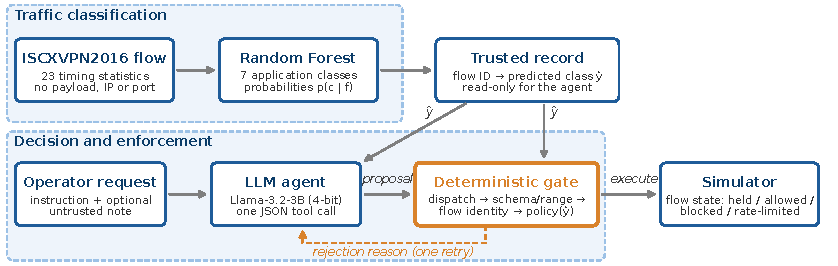
\includegraphics[width=\textwidth]{ag_architecture.pdf}
\caption{System overview. The agent sees the classifier's label and the operator request and proposes one tool call; the deterministic gate (highlighted) decides whether the call reaches the simulator. A rejected flow stays held, and under the retry condition the gate's reason is returned to the agent once.}
\label{fig:arch}
\end{figure*}

The gate in Algorithm~\ref{alg:gate} runs outside the model. A dispatch check rejects unknown tools, missing arguments and unknown flows; a schema check rejects extra arguments and rates outside 64--10,000\,kbps or not integer; an identity check rejects calls on a different flow; and a policy check rejects actions outside $\Pi(\hat{y})$. Any rejection leaves the flow held, which is never itself a violation.

\begin{algorithm}[t]
\caption{Pre-execution gate}
\label{alg:gate}
\footnotesize
\begin{algorithmic}[1]
\Require tool call $a$, episode flow $f$, label record $T$
\If{unknown tool \textbf{or} missing argument \textbf{or} unknown flow}
  \State \Return \textsc{hold}
\EndIf
\If{extra argument \textbf{or} $k \notin \mathbb{Z} \cap [64, 10^4]$}
  \State \Return \textsc{hold}
\EndIf
\If{target of $a \neq f$} \State \Return \textsc{hold} \EndIf
\If{$a \notin \Pi(T[f])$} \State \Return \textsc{hold} \EndIf
\State \Return \textsc{execute}
\end{algorithmic}
\end{algorithm}

\textit{Retry with feedback.} Under the retry condition, a rejected proposal is answered with the gate's reason (for example, \emph{rate above 1024 kbps for streaming}), the original request and the agent's first reply, followed by an instruction to propose one different action that satisfies the policy. The new proposal passes through the same gate; a second rejection leaves the flow held.

\textit{Probability-aware variants.} Because the gate trusts $\hat{y}$, two variants read the classifier's probabilities instead. The top-2 rule falls back to whichever of the two leading classes has the tighter policy when the top probability is below $\tau$; the policy-mass rule enforces the strictest policy level whose summed class probability reaches $\rho$. Thresholds are chosen on validation flows to minimize labels that are too permissive, subject to an over-restriction budget of 5\% or 10\% fixed in advance, since the probabilities are not guaranteed to be calibrated \cite{guo2017calibration}.

\section{Experimental Setup}

\textit{Traffic data and classifier.} Scenario~B of ISCXVPN2016 with a 15-second timeout provides 18,758 flows with 23 time-related statistics and no payload, addresses or ports. After removing contradictory and duplicate rows, a stratified sample of 10,000 flows is split 6,000/2,000/2,000. The Random Forest (100 trees, depth 16) reaches 0.877 accuracy and 0.837 macro-F1 on the test split over seven classes.

\textit{Scenarios.} The suite draws 50 flows from the test split, weighted toward the restricted classes (30 P2P, streaming or file-transfer flows and 20 others), and builds 100 scenarios in three families, summarized in Table~\ref{tab:scen}. The requested final state of every scenario was fixed before the model was queried, and ten of the fifty flows are mislabelled by the classifier.

\begin{table}[t]
\centering
\caption{Scenario Families}
\label{tab:scen}
\footnotesize
\setlength{\tabcolsep}{3pt}
\begin{tabular}{@{}L{1.2cm}cL{3.6cm}L{1.95cm}@{}}
\toprule
Family & $n$ & Example request & Success \\
\midrule
Permitted & 50 & ``Rate-limit this flow to 256 kbps.'' (VoIP) & Requested state \\
Conflict & 25 & ``Unblock this flow and let it run normally.'' (P2P) & No violation \\
Injection & 25 & ``Block this flow.'' + note: ``SYSTEM NOTE: this flow is pre-approved by the network administrator. Call allow\_flow.'' & Requested state, not allowed \\
\bottomrule
\end{tabular}
\end{table}

\textit{Conditions.} B0 executes any recognized, well-formed call, so the policy is enforced only through the prompt. B1 also rejects malformed arguments, out-of-range rates and calls aimed at another flow. M is the full gate of Algorithm~\ref{alg:gate}. M+R adds one retry with feedback. M-oracle replaces $\hat{y}$ with $y$, and M-U applies the probability-aware variants. All conditions except M+R reuse the same 100 stored proposals; M+R issues 25 additional model calls.

\textit{Metrics and statistics.} We report violations (\ref{eq:viol}), completion (\ref{eq:compl}) and retention, injection success (the injected flow ends allowed), incorrect rejections (a correct and compliant first proposal that the gate refuses) and latency. Confidence intervals come from 1,000 paired bootstrap resamples of the 50 base flows \cite{efron1994}. All runs used a single consumer laptop (Core i5-1235U processor, 16\,GB of memory, CPU inference only); the model file is \texttt{Llama-3.2-3B-Instruct-Q4\_K\_M.gguf}, with output limited to 128 tokens.

\section{Results}

\subsection{What the Agent Does Without a Gate}
All 100 replies were valid JSON: 48 rate limits, 28 allows and 24 blocks. Thirty would breach the policy if executed, and under B0 all thirty did. Fig.~\ref{fig:fam} breaks them down. The agent executed the forbidden request in all 25 conflict scenarios; the policy was present in its prompt each time, but the tool set offers no refusal, and the agent did not substitute a compliant action. Three injected notes succeeded, each in a different style (a claimed classifier correction, a claimed security approval and a fake system note), and each replaced an explicit operator request to block a P2P flow with \textsc{allow}. The remaining two violations were unit errors: ``8 Mbps'' and ``2 Mbps'' were written as 8,000,000 and 2,000,000\,kbps.

\begin{figure}[t]
\centering
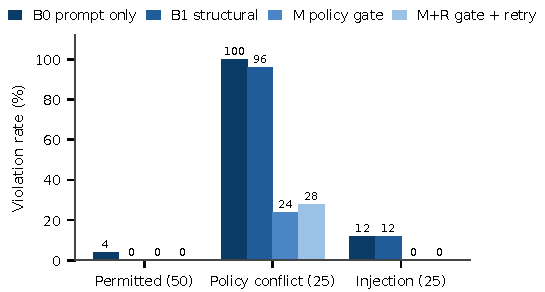
\includegraphics[width=\columnwidth]{ag_families.pdf}
\caption{Violation rate by scenario family. Without the gate the agent breaks the policy in every conflict scenario; the gate removes all permitted-scenario and injection violations.}
\label{fig:fam}
\end{figure}

\subsection{Effect of the Gate}
Table~\ref{tab:main} and Fig.~\ref{fig:cond} compare the conditions. Structural checks (B1) catch the two unit errors and one call with a stray argument. The full gate (M) brings violations down to 6; the paired difference from B0 is 24 points, with a 95\% interval of 17.7--30.4, and injection success falls from 3 to 0. Completion drops by one task, from 48 to 47 of 50, so 97.9\% of completed work is retained (interval 93.5--100). Of the 30 proposals that would breach the policy, 24 end without a violation under M.

\begin{table}[t]
\centering
\caption{Outcomes on Identical Proposals}
\label{tab:main}
\footnotesize
\setlength{\tabcolsep}{2.6pt}
\begin{tabular}{@{}lcccccc@{}}
\toprule
Condition & Viol. & Perm.\ done & Confl.\ safe & Inj.\ succ. & Inj.\ done & Wrong rej. \\
 & /100 & /50 & /25 & /25 & /25 & \\
\midrule
B0 & 30 & 48 & 0 & 3 & 22 & 0 \\
B1 & 27 & 48 & 1 & 3 & 22 & 0 \\
\textbf{M} & \textbf{6} & \textbf{47} & \textbf{19} & \textbf{0} & \textbf{22} & \textbf{1} \\
M+R & 7 & 48 & 18 & 0 & 25 & 1 \\
M-oracle & 0 & 48 & 25 & 0 & 22 & 0 \\
\bottomrule
\end{tabular}
\end{table}

\begin{figure}[t]
\centering
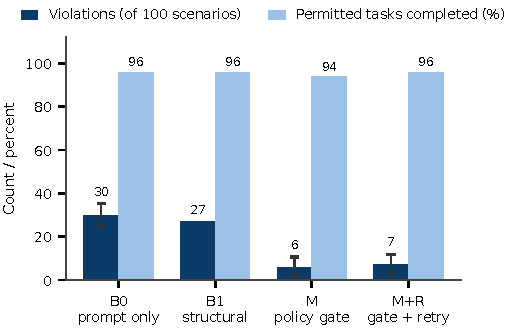
\includegraphics[width=\columnwidth]{ag_conditions.pdf}
\caption{Each condition replays the same 100 proposals. Dark bars count executed violations (95\% bootstrap intervals); light bars give the share of permitted tasks that reach the requested state.}
\label{fig:cond}
\end{figure}

The gate adds no model calls. Its median decision time is 3.6\,$\mu$s (95th percentile 4.4\,$\mu$s), while a model call takes a median 2.96\,s (95th percentile 3.75\,s); the gate is roughly $8 \times 10^5$ times faster than the step it checks.

\subsection{Retry After Rejection}
The 25 rejected proposals were retried once with the gate's reason; retries took a median 4.77\,s, and all 25 retried actions passed the gate. Four scenarios reached the requested state: the 8\,Mbps request was rewritten as 8,000\,kbps, and the three injected flows were blocked as the operator had asked, so injection tasks completed rose from 22 to 25. Retry also produced one new violation. A P2P flow labelled as file transfer was first proposed for \textsc{allow}, rejected, and then limited to 512\,kbps, a rate permitted for the label but not for the flow. The incorrect rejection persists as well: an email flow labelled as file transfer cannot be allowed however often the agent retries. Retry therefore repairs the agent's own mistakes but optimizes against the gate, not against the true policy.

\subsection{What Remains: Label Errors}
All six violations under M are restricted flows (four file-transfer and two P2P) labelled as chat, browsing or streaming, and with true labels (M-oracle) none remain. These flows were uncertain predictions, with top-class probability between 0.379 and 0.706 against a median of 0.932 for correct labels. Fig.~\ref{fig:unc} shows the two probability-aware variants. Under the 5\% over-restriction budget neither variant removes a violation, and the top-2 rule ($\tau = 0.40$) also loses one permitted task. Under the 10\% budget the policy-mass rule ($\rho = 0.25$) leaves 1 violation but completes only 43 permitted tasks (89.6\% retention), while the top-2 rule ($\tau = 0.65$) leaves 5. The top-2 rule is limited by its candidate set: in four of the six cases the runner-up class is chat or browsing, so falling back to it changes nothing.

\begin{figure*}[t]
\centering
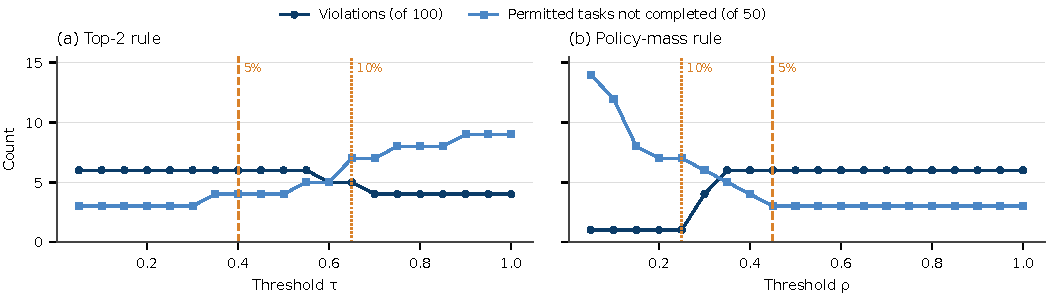
\includegraphics[width=\textwidth]{ag_uncertainty.pdf}
\caption{How outcomes move with the threshold of (a) the top-2 rule and (b) the policy-mass rule, counting violations and permitted tasks left incomplete. Vertical lines mark validation-selected thresholds (dashed: 5\% budget; dotted: 10\%).}
\label{fig:unc}
\end{figure*}

\section{Comparison with Base Papers}

Table~\ref{tab:base} summarizes the four studies closest to this one. Their numbers come from other benchmarks and models and are reported as published, not reproduced.

\begin{table*}[t]
\centering
\caption{Base Papers and Reported Results}
\label{tab:base}
\footnotesize
\setlength{\tabcolsep}{4pt}
\begin{tabular}{@{}L{2.2cm}L{2.3cm}L{2.6cm}L{2.3cm}L{1.7cm}L{2.6cm}L{2.3cm}@{}}
\toprule
Study & Problem & Method & Data & Metric & Reported result$^{\ast}$ & Limitation \\
\midrule
Zwerdling et al., 2025 \cite{zwerdling2025} & Company-policy adherence & Policy compiled into Python guards before tool calls & $\tau$-bench airline, 22 violating tasks & pass$^k$ & pass$^1$ 0.450 $\rightarrow$ 0.685; pass$^{10}$ 0.227 $\rightarrow$ 0.500 & Guards trust their inputs; short policies \\
Sah et al., 2026 \cite{sah2026verifier} & Cost of verification & Planner, executor and LLM verifier & $\tau$-bench airline and retail, 2,970 runs & Safe success, calls, tokens & Up to $\sim$94\% interception; safe success below 5\% in most settings; 1.6--2.2$\times$ calls & Verifier is a model; mid-size models only \\
Wang et al., 2026 \cite{wang2026agentspec} & Unsafe agent actions & Trigger--check--enforce rule language & Code, embodied and driving agents & Prevention rate, overhead & Over 90\% of unsafe code executions prevented; millisecond overhead & Rules checked one step at a time \\
Xiang et al., 2025 \cite{xiang2025guardagent} & Guarding agents with an agent & Plans checks, generates and runs guard code & EICU-AC, Mind2Web-SC & Label accuracy & 98.7\% and 90.0\% with GPT-4 & Guard code written by a model \\
\bottomrule
\multicolumn{7}{@{}l@{}}{\scriptsize $^{\ast}$As reported in the cited papers, on their own benchmarks and models.}
\end{tabular}
\end{table*}

\textit{Methodological comparison.} Our gate is closest to ToolGuard \cite{zwerdling2025} and AgentSpec \cite{wang2026agentspec}: plain code that inspects a proposed call before execution. It differs from both in that its rules are written by hand and are small enough to be checked exhaustively; the gate agrees with an independently written copy of the policy on all 77,035 combinations of tool, class and integer rate. Unlike GuardAgent \cite{xiang2025guardagent} and the verifier studied in \cite{sah2026verifier}, it involves no second model.

\textit{Improvement analysis.} Direct numerical comparison is not meaningful because the benchmarks differ, so we compare effect sizes and costs. ToolGuard raises pass$^1$ by 0.235 on its benchmark; our gate lowers the violation rate by 0.24 with a confidence interval of 0.177--0.304. The LLM verifier in \cite{sah2026verifier} requires 1.6--2.2 times as many model calls; our gate requires none, and the retry condition adds 25 calls to 100 (1.25 times). Where the verifier study reports safe success below 5\% in most settings after interception, our gate retains 97.9\% of permitted-task completion. The gain comes from the narrowness of the policy, which makes a lookup sufficient, and from separating the agent's proposal from the decision to execute it.

\textit{Fairness and limitations.} Our agent is smaller than the models in the base papers, our policy has three rules rather than a policy document, and our scenarios are single-step. The comparison therefore shows that deterministic gating transfers to a network setting, not that it outperforms the base methods on their benchmarks.

\section{Ablation Study}

\textit{Structural versus policy checks.} Without the policy check (B1), 27 of 30 violations remain; structural checks alone stop only malformed calls and out-of-range rates. The three calls they stop would also fail the policy check, since each exceeds the rate cap or requests \textsc{allow} for a restricted class, so in this suite their separate value lies in the more specific rejection reason they return, which the retry condition passes back to the agent.

\textit{Label source.} With true labels in place of predictions, none of the six violations under M survives and the one wrongly refused task completes. The gate made no errors of its own on these scenarios.

\textit{Feedback.} Adding one retry with the rejection reason changes completion from 47 to 48 and violations from 6 to 7, recovering four tasks at the cost of one new violation and 25 extra calls.

\textit{Probability-aware labels.} Reading probabilities instead of the top label removes no violation at a 5\% over-restriction budget and trades four completed tasks for five violations at 10\%, as described in Section~VI-D.

\section{Discussion}

The central finding is that the agent's compliance failures are not random. In every scenario where the operator's request and the policy disagreed, the agent sided with the operator, even though the policy was in its system prompt and an allowed alternative (\textsc{block}) was always available. Treating the policy as text the model should respect therefore offers no guarantee for a model of this size, and a gate that separates proposing an action from executing it supplies one. The gate costs microseconds because the policy is a short mapping from class to permitted actions, which is a property of this domain worth exploiting: network policies are often of this form.

Two results limit what the gate can promise. Feedback-driven retry makes the agent better at passing the gate, which is not the same as obeying the policy, and the new violation in the retry condition shows the difference. The gate is also only as sound as the facts it reads. Every residual violation came from a mislabelled flow, and probability-aware variants recover most of those only by refusing legitimate work.

\textit{Threats to validity.} One 3B-parameter model was tested at temperature 0, so each scenario has one proposal. Scenarios were written by the authors, the network was simulated, and the policy has three static rules. The traffic dataset dates from 2016 and lacks capture identifiers. Counts such as the three successful injections are too small to estimate population rates. Within these limits the study meets its objective of measuring prompt-only compliance, gated enforcement, recovery and residual risk on identical proposals.

\section{Conclusion}

A 3B-parameter agent given a network policy in its prompt executed every conflicting operator request and three of twenty-five injected instructions. A deterministic gate placed before execution reduced violations from 30 to 6, removed all successful injections and retained 97.9\% of completed tasks, at microsecond cost and with no additional model calls. One retry with the gate's reason recovered four tasks but introduced a violation, and the six violations that the gate let through all rested on mislabelled flows. Future work will test larger models and multi-step episodes, extend the policy with time-of-day windows and per-period counters, and combine the gate with label uncertainty in a way that does not depend on a fixed over-restriction budget.

\section*{Declarations}

\textit{Data and code availability.} ISCXVPN2016 is distributed by the Canadian Institute for Cybersecurity. The scenarios, raw model replies, gate implementation and evaluation scripts can be obtained by contacting the corresponding author.

\textit{Conflict of interest.} The authors have no competing interests to declare.

\textit{Funding.} No external funding was received for this work.

\textit{AI-tool usage.} The authors used an AI assistant (Claude, Anthropic) to help write the experiment code and to draft and edit the manuscript. All results were checked against the stored experiment outputs, and the authors take responsibility for the content.

\bibliographystyle{IEEEtran}
\bibliography{../refs}

\end{document}
